\chapter{THE REVERSE MAPPING PROBLEM}
\thispagestyle{plain}

\label{ReverseMapping}

POINT vs. SPACE. What information does a point give? not much. a space gives lots of information!


Lorem ipsum dolor sit amet, consectetur adipisicing elit, sed do eiusmod tempor incididunt ut labore et dolore magna aliqua. Ut enim ad minim veniam, quis nostrud exercitation ullamco laboris nisi ut aliquip ex ea commodo consequat. Duis aute irure dolor in reprehenderit in voluptate velit esse cillum dolore eu fugiat nulla pariatur. Excepteur sint occaecat cupidatat non proident, sunt in culpa qui officia deserunt mollit anim id est laborum.

For example, suppose we want to find the configurations in Sheep Wolf Predation that produce an average of 100 sheep.
First, assume that a forward-mapping surface $\vec{s} : f(\mathbf x) = \hat y$ has been learned.
This surface represents the behavior space: mapping configuration vectors (denoted by the vector $\mathbf x$) to a predicted system-level property (the average number of sheep; denoted by $\hat y$).
For this example, $\hat y = 100$.
In many cases, solving for $\mathbf x$ in the equality $\mathbf x) = \hat y$ is difficult.\footnote{More on the difficulties in this problem are presented in Chapter \ref{ReverseMapping}: The Reverse Mapping Problem}
An alternative method than solving this problem anaytically is to use SSI algorithms to determine the intersection between a surface $\vec{p} : \hat y = 100$  and $\vec{s}$.
The intersection found will represent the complete set of configurations that would generate the behavior $\hat y$.

\begin{figure}[ht]
\centering
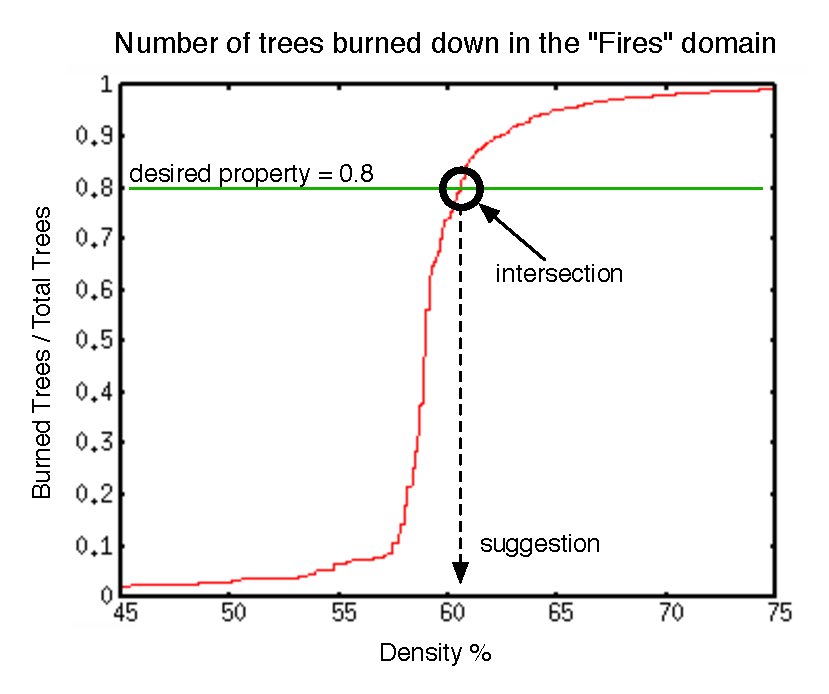
\includegraphics[scale=.66667]{images/firespace-intersection.pdf}
\caption{An illustration of using surface-to-surface intersection to solve the reverse-mapping problem in the NetLogo Fires domain.}
\label{fig:fires-inter}
\end{figure}

The Wolf Sheep behavior space is highly dimensional due to the number of configuration paramethers.
Therefore, visualizing the previous example is difficult.
For the sake of example, consider the simple NetLogo Fires domain\footnote{This domain is analyzed in detail in Subsection \ref{sec:Fires}} \cite{fires}.
This domain only has one configuration parameter: the density percentage of the number of trees ($x$).
The system-level property being measured is the percentage of trees that were burned down ($\hat y$).
Therefore, the behavior space is two-dimensional and the surface is a simple sigmoid-like curve.
This curve is plotted in Figure \ref{fig:fires-inter}.
To frame this as an SSI problem in order to find the configuration that cause the system to exhibit 80\% of its trees burned down, \fw finds the intersection between the line $y = 0.8$ and the behavior space curve.
Once this intersection is found with an SSI algorithm, the configuration suggestion can be extracted as the solution to the reverse mapping problem.
